\subsection{Final selection with updated ECAL calibration}
\label{sec:enujjFinalSelectionUpdate}

One of the 5 events (run 178708, luminosity section 326, event number 532162137) 
passing the \enujj~final selection for LQ mass of 850 GeV reported 
in Table~\ref{tab:enujjFinalSelection} is affected by a serious calibration problem 
in one EE channel.  This channel reports a calibration coefficient
with a value greater than 3.0, while the expected value is 1.0.
The calibration problem is present in the conditions used to reconstruct
the dataset /ElectronHad/Run2011B-PromptReco-v1/AOD
listed in Table~\ref{tab:SingleElectronPlusElectronHadDataset}, which has 
been used to produce the \enujj~analysis results shown so far.
It is likely that this event contains a real electron with \pt~of about 200~\GeV.
The electron in this event is measured by the EE channel affected by the problem.  
Due to the wrong calibration factor, the electron \pt~is incorrectly reconstructed at 
approximately 550~\GeV. This mismeasured electron generates mismeasured \MET~(approximately 400~\GeV) 
on the opposite side (in $\phi$) of the detector. 
An event display highlighting this event is shown in Figure~\ref{fig:problematicEvent} (left).

This calibration problem was identified and fixed in a re-reconstruction of the data
that was made available at the end of November 2011, known as the "Nov30" re-reconstruction.
An event display highlighting this event under the Nov30 re-reconstruction is shown in Figure~\ref{fig:problematicEvent} (right).
In the Nov30 re-reconstruction, the electron \pt~for this event is reduced 
significantly compared to the value from the original reconstruction,
and the \MET~is now about 40~\GeV. Under the Nov30 re-reconstruction,
the event does not even pass the \enujj~preselection. 

\begin{figure}[htbp]
  \begin{center}
    \begin{tabular}{cc}
      \resizebox{7.5cm}{!}{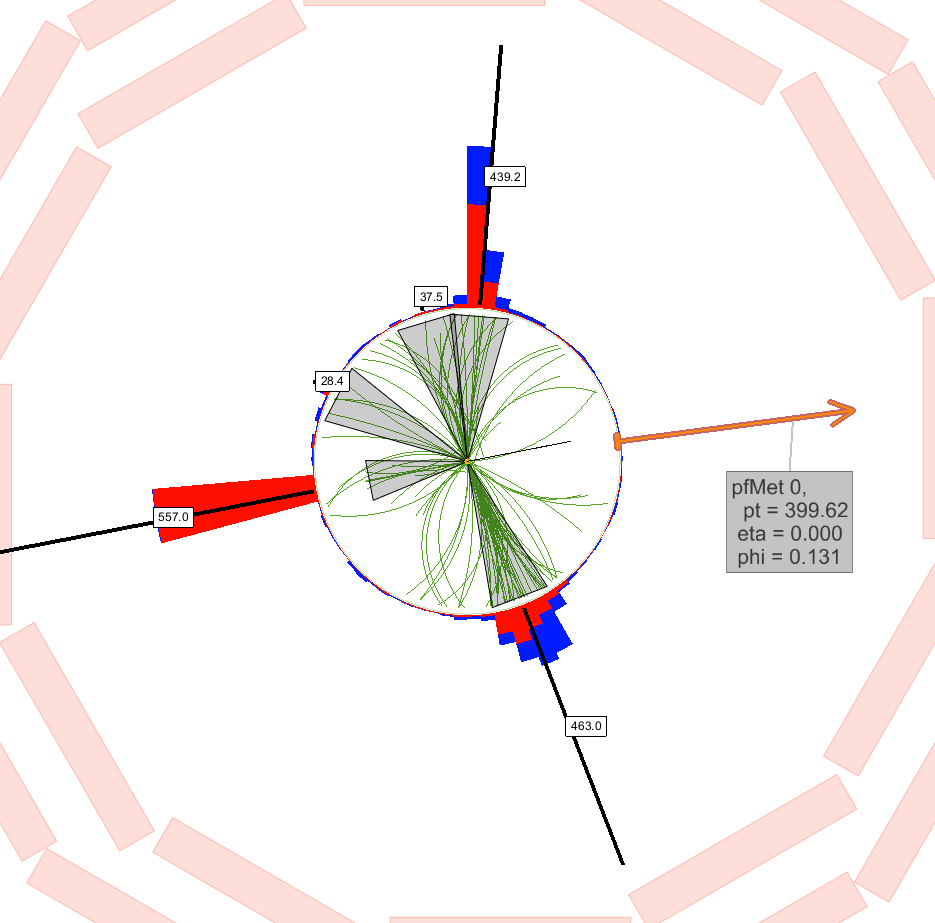
\includegraphics{tex/analysis/event_selection/fig/event_display/old_reco-178708_532162137_326_RhoPhi.png}} &
      \resizebox{7.5cm}{!}{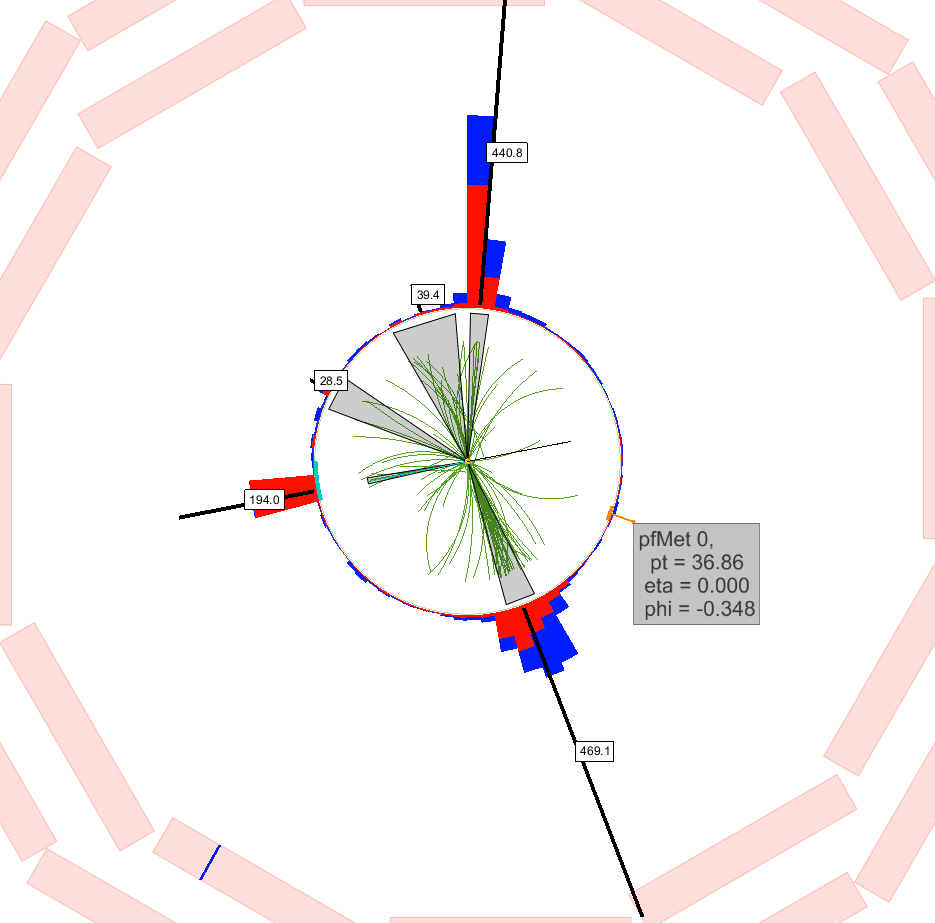
\includegraphics{tex/analysis/event_selection/fig/event_display/new_rereco-178708_532162137_326_RhoPhi.png}} \\
    \end{tabular}
    \caption{Event displays showing the event discussed in this section 
      [run 178708, luminosity section 326, event number 532162137] as reconstructed in the original reconstruction (left) and in the
      Nov30 re-reconstruction (right).
      An ECAL calibration problem that affected this event in the original reconstruction 
      was fixed in the Nov30 re-reconstruction.
      The electron affected by the calibration problem is represented as a red energy cluster in the ECAL
      on the left side of both event displays.
      The \met~measurement is represented as a red arrow on the right side of both event displays.
    }
    \label{fig:problematicEvent}
  \end{center}
\end{figure}

Unfortunately, the ElectronHad dataset used \enujj~channel (see Table~\ref{tab:SingleElectronPlusElectronHadDataset})
was not centrally reprocessed under the Nov30 re-reconstruction.
Therefore, the 1576 events in data that pass 
the \enujj~selection optimized for a LQ with mass of 250 \GeV~(see 
Table~\ref{tab:enujjFinalSelection})
were privately reprocessed using the conditions from the Nov30 re-reconstruction.

This section presents the results of the final \enujj~selection in the same 
format reported in Section~\ref{sec:enujjFinalSelection}, but 
using the 1576 events in data that were privately re-reconstructed.
The background predictions remain unchanged.
The bias introduced by the fact that the 
whole ElectronHad dataset has not been reprocessed is negligible 
in this case. 
It is much more likely that 1 (originally common) background-like event would be promoted to pass 
the \enujj~final selection due to a similar calibration problem than it is likely that
1 (rare) signal-like event is removed from the final selection.
This is because there are many more background-like events than signal-like events.
It is expected, therefore, that the main effect will be to see fewer events 
passing the \enujj~selection criteria in the private re-reconstruction than in the original reconstruction.
In addition, because the presence of fake \MET~is 
a typical consequence of an electron measurement problem, the \eejj~channel (where no \MET~requirement is applied) 
is believed to be unaffected. As a cross check, 
the 6 events passing the final \eejj~selection optimized for LQ mass of 650 \GeV~(see 
Table~\ref{tab:eejjFinalSelection}) were also privately re-reconstructed;
no significant difference between the private re-reconstruction and the original reconstruction was observed.
     
Table~\ref{tab:enujjFinalSelection_Nov30} shows the number of events
for the data, the backgrounds, and the LQ signal, after applying the final, optimized \enujj~selection 
criteria summarized in Table~\ref{tab:enujjOptimizedCuts}.
Figures~\ref{fig:st_mej_fullSelection400_enujj_Nov30} and~\ref{fig:st_mej_fullSelection600_enujj_Nov30} 
show the distributions of \st~and the selected electron-jet invariant mass, \mej, after the full selection 
optimized for \MLQ$=400$ and 600~\GeV, respectively. 
The dominant background contributions are from \ttbar~sand \wjets~events, 
while the contribution from the other backgrounds is below \OtherBackgroundContributionINenujj~for 
the leptoquark masses within the current reach of this analysis. 
A good agreement is observed between the data and the background 
prediction within statistical uncertainties.    

As expected, the event affected by the calibration problem (run 178708, luminosity section 326, event number 532162137)
is removed from the final \enujj~selection with the new ECAL calibration.
For the other events, there are only minor changes between the results 
shown in Section~\ref{sec:enujjFinalSelection} and those presented here.

\begin{table} 
  \small 
  \begin{tabular}{l | c | c | c | c | c | c | c} 
    $M_{LQ}$ & LQ Signal & W+Jets & $t\bar{t}$ & QCD & Other & Data &  Total BG \\ 
    \hline 
    \hline 
    250    & $ 1703.5 \pm 13.8 $   &  $ 190  \pm 9.2  $ & $ 195  \pm 6.2  $ & $ 31.7  \pm 1.2  $  & $ 43.3 \pm 2.19 $ &430 & $ 460.4 \pm 11.4 $ \\ 
    350    & $ 285.54 \pm 2.06 $   &  $ 52.1 \pm 4.8  $ & $ 34.2 \pm 2.6  $ & $ 15.2  \pm 0.97 $  & $ 10.9 \pm 0.92 $ &92 & $ 112.4 \pm 5.6 $ \\ 
    400    & $ 126.01 \pm 0.82 $   &  $ 28.7 \pm 3.6  $ & $ 17.5 \pm 1.8  $ & $ 6.20  \pm 0.46 $  & $ 6.01 \pm 0.77 $ &43 & $ 58.4 \pm 4.1 $ \\ 
    450    & $ 68.38 \pm 0.43 $    &  $ 19.7 \pm 2.9  $ & $ 12.2 \pm 1.5  $ & $ 3.01  \pm 0.31 $  & $ 4.13 \pm 0.44 $ &29 & $ 39.1 \pm 3.3 $ \\ 
    500    & $ 34.70 \pm 0.23 $    &  $ 13.3 \pm 2.4  $ & $ 6.3  \pm 1.1  $ & $ 1.72  \pm 0.22 $  & $ 2.80 \pm 0.37 $ &18 & $ 24.2 \pm 2.6 $ \\ 
    550    & $ 16.25 \pm 0.10 $    &  $ 2.98 \pm 0.95 $ & $ 3.38 \pm 0.82 $ & $ 0.65  \pm 0.10 $  & $ 1.46 \pm 0.26 $ &10 & $ 8.5 \pm 1.3 $ \\ 
    600    & $ 9.442 \pm 0.056 $   &  $ 2.45 \pm 0.87 $ & $ 2.33 \pm 0.67 $ & $ 0.57  \pm 0.10 $  & $ 1.29 \pm 0.25 $ &6 & $ 6.6 \pm 1.1 $ \\ 
    650    & $ 5.202 \pm 0.032 $   &  $ 2.03 \pm 0.83 $ & $ 1.01 \pm 0.41 $ & $ 0.335 \pm 0.079 $ & $ 0.76 \pm 0.20 $ &4 & $ 4.14 \pm 0.95 $ \\ 
    750    & $ 1.851 \pm 0.010 $   &  $ 1.45 \pm 0.65 $ & $ 0.62 \pm 0.31 $ & $ 0.287 \pm 0.080 $ & $ 0.65 \pm 0.18 $ &4 & $ 3.01 \pm 0.75 $ \\ 
    850    & $ 0.6973 \pm 0.0037 $ &  $ 1.22 \pm 0.61 $ & $ 0.62 \pm 0.31 $ & $ 0.251 \pm 0.078 $ & $ 0.61 \pm 0.19 $ &4 & $ 2.70 \pm 0.71 $ \\ 
  \end{tabular}
  \caption{Number of events after the final \enujj~selection following a private re-reconstruction. 
    Only statistical uncertainties are reported.}
  \label{tab:enujjFinalSelection_Nov30}
\end{table}

\begin{figure}
  \begin{center}
    \begin{tabular}{cc}
      \resizebox{7.5cm}{!}{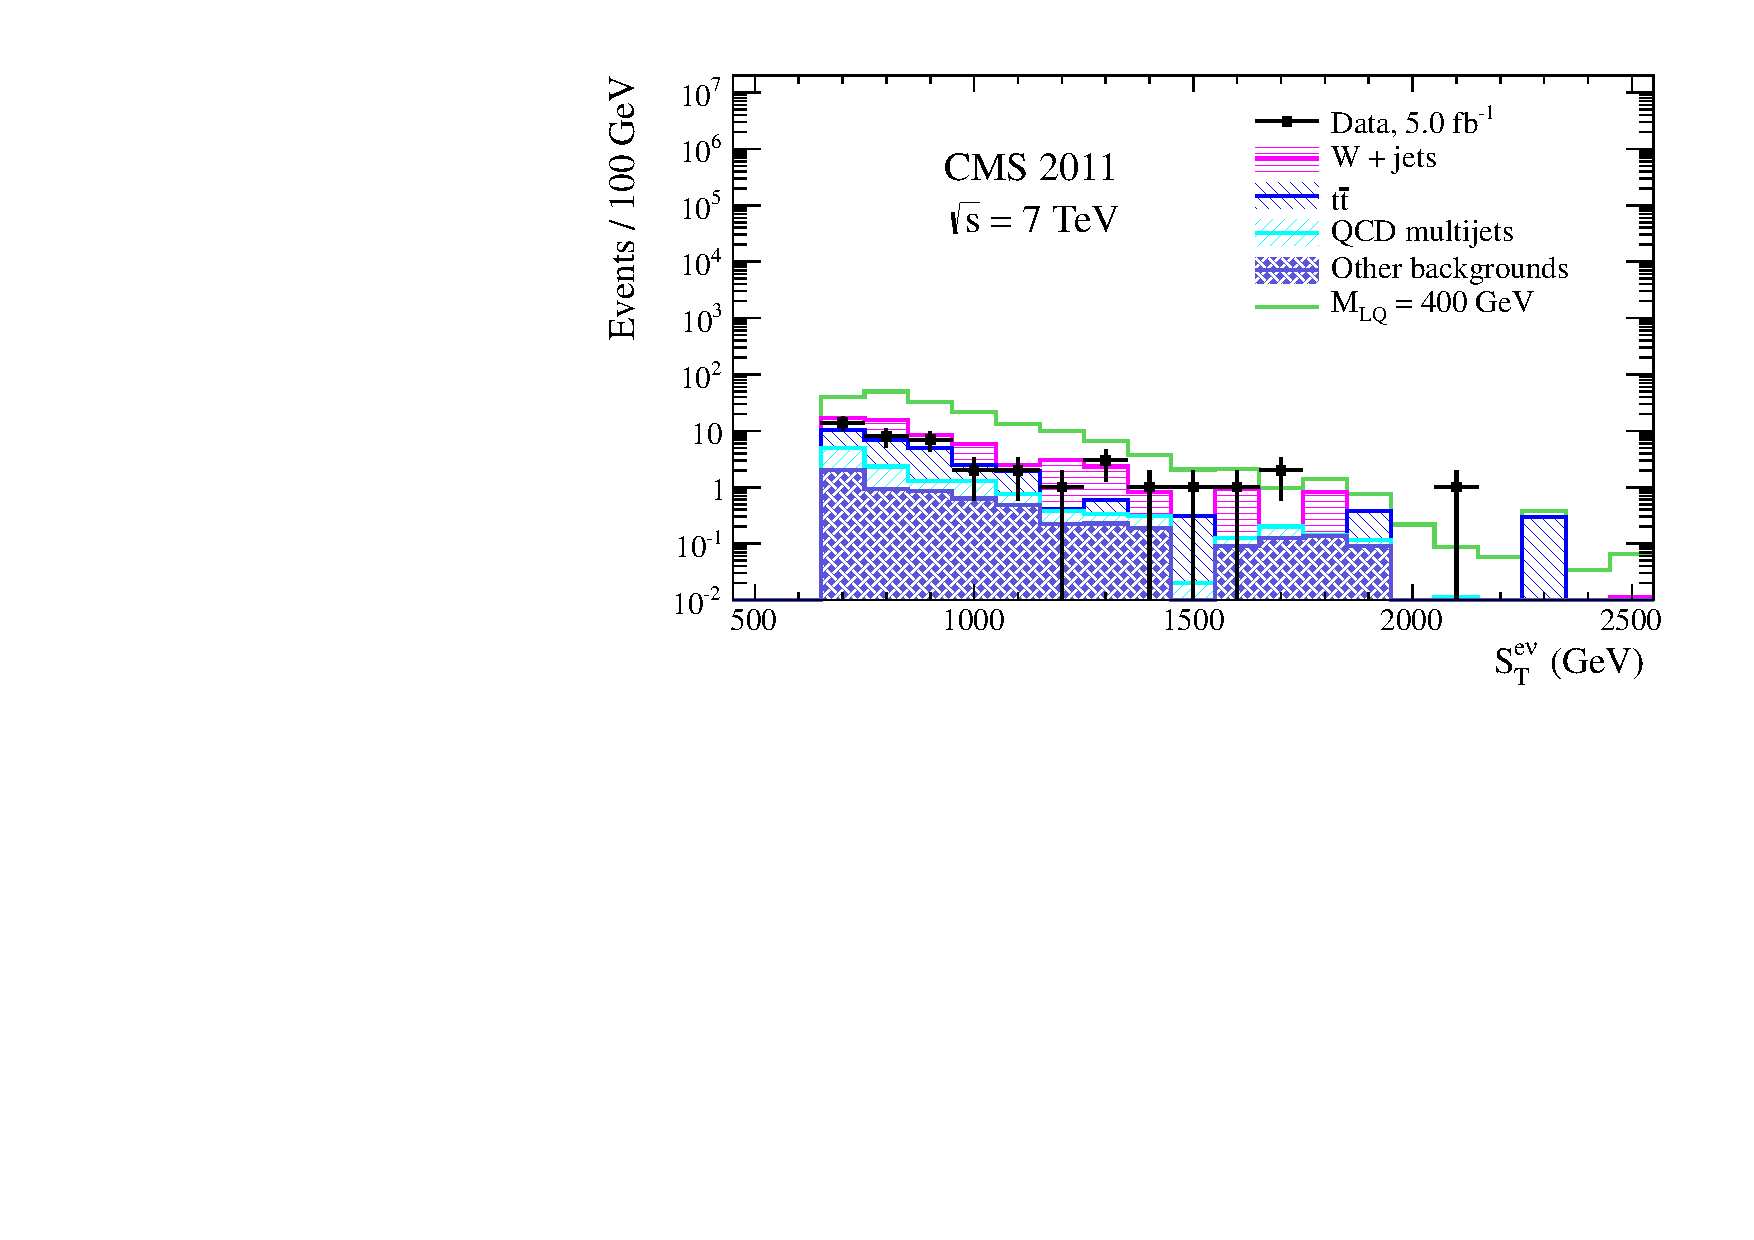
\includegraphics{tex/analysis/event_selection/fig/enu/final_selection_update/sT_LQ400_enujj_WZSherpa_MT120_NewRereco.pdf}} &
      \resizebox{7.5cm}{!}{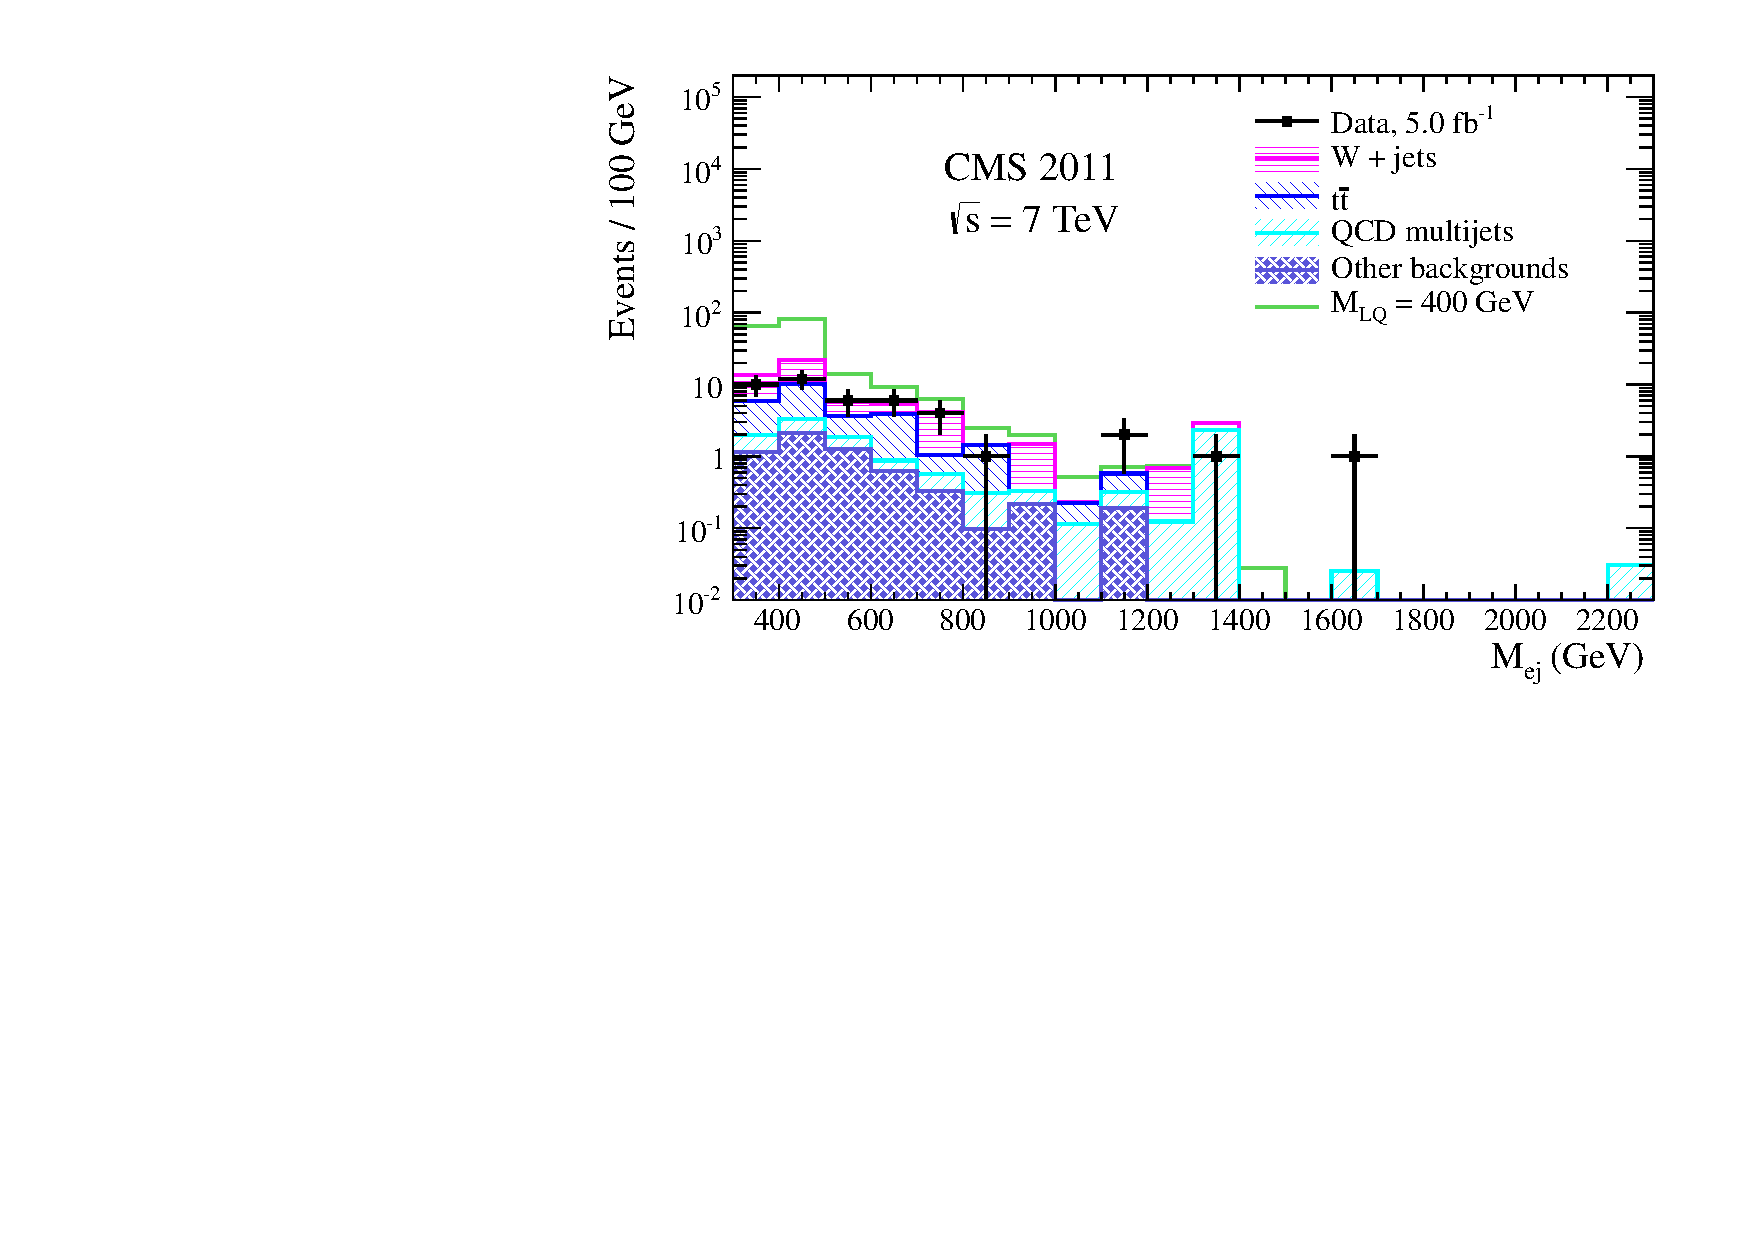
\includegraphics{tex/analysis/event_selection/fig/enu/final_selection_update/Mej_LQ400_enujj_WZSherpa_MT120_NewRereco.pdf}} \\
    \end{tabular}
    \caption{The \st (left)
             and \mej (right) distributions 
             for events passing the full \enujj selection optimized for \MLQ$=400$~\GeV. Nov30 conditions are used for the data.}
    \label{fig:st_mej_fullSelection400_enujj_Nov30}
  \end{center}
\end{figure}

\begin{figure}
  \begin{center}
    \begin{tabular}{cc}
      \resizebox{7.5cm}{!}{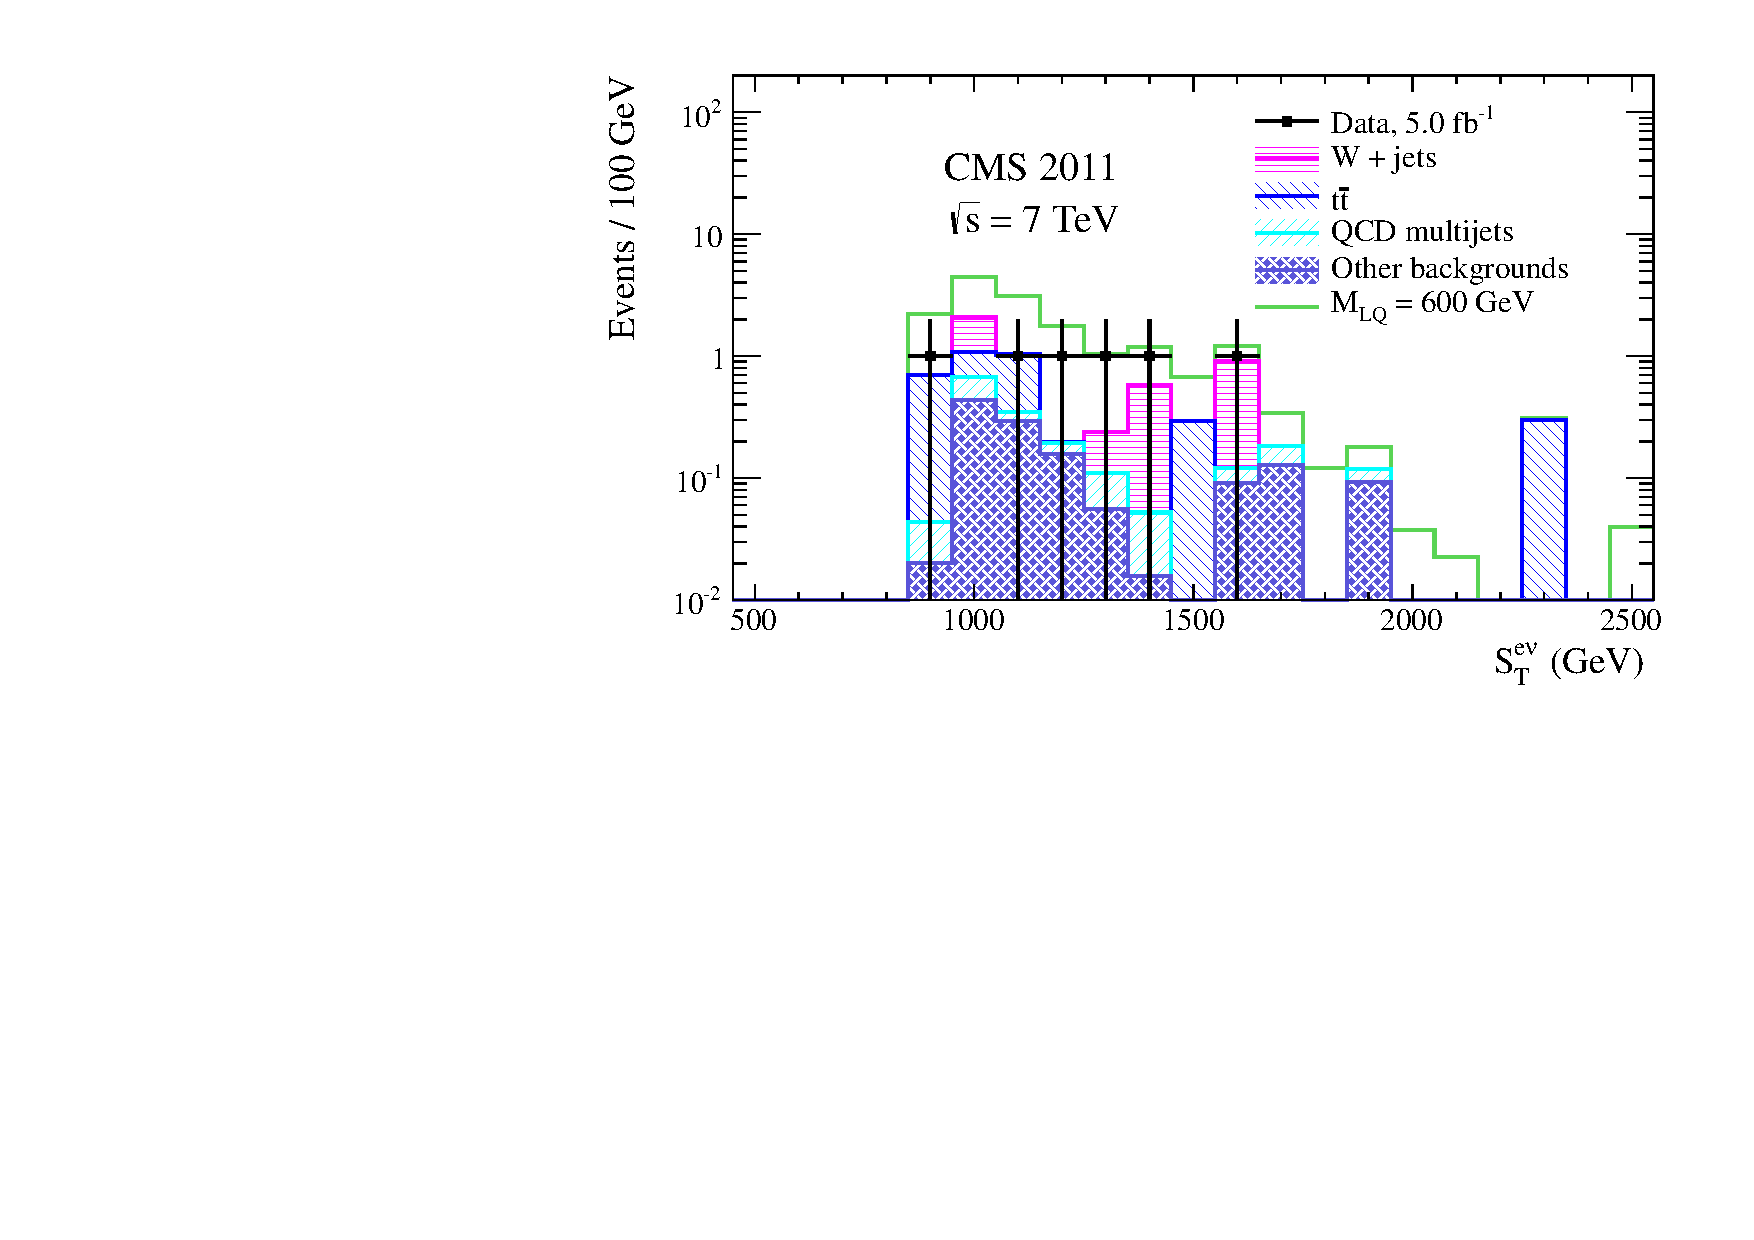
\includegraphics{tex/analysis/event_selection/fig/enu/final_selection_update/sT_LQ600_enujj_WZSherpa_MT120_NewRereco.pdf}} &
      \resizebox{7.5cm}{!}{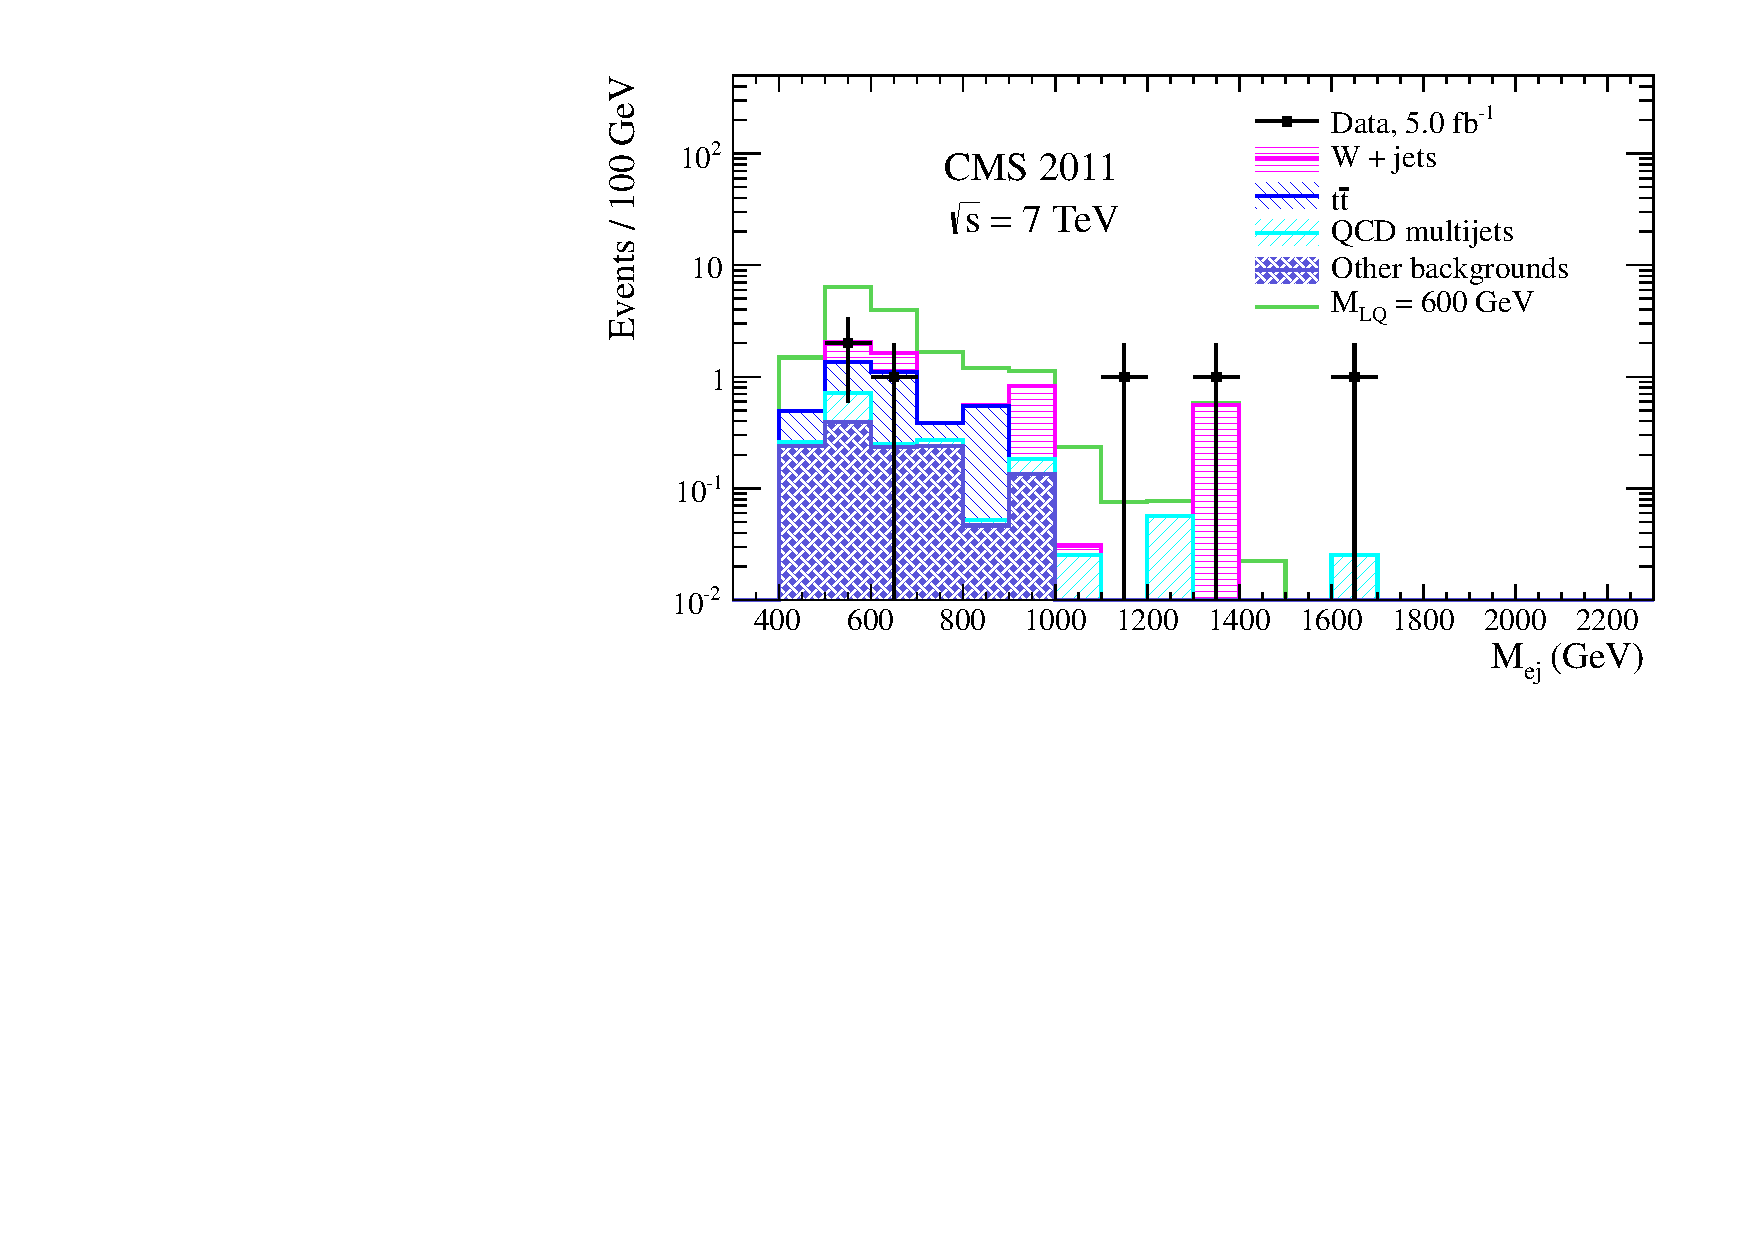
\includegraphics{tex/analysis/event_selection/fig/enu/final_selection_update/Mej_LQ600_enujj_WZSherpa_MT120_NewRereco.pdf}} \\
    \end{tabular}
    \caption{The \st (left)
             and \mej (right) distributions 
             for events passing the full \enujj selection optimized for \MLQ$=600$~\GeV. Nov30 conditions are used for the data.}
    \label{fig:st_mej_fullSelection600_enujj_Nov30}
  \end{center}
\end{figure}
